\documentclass[12pt]{report}
\usepackage[margin=3cm]{geometry}
\usepackage[T1]{fontenc}
\usepackage{amsmath}
\usepackage{mathabx}
\usepackage{tikz}
\usepackage{capt-of}
\usepackage{setspace}
\usepackage{titlesec}
\usepackage{ragged2e}
\usepackage{graphicx}
\usepackage{float}

\title{Belove nejednakosti\\
{\Large Univerzitet u Banjoj Luci}\\
{\Large Prirodno-matematički fakultet}}
\author{Stefani Tovilović}
\date{September 2023}

\setstretch{1.5}

\begin{document}

\renewcommand{\contentsname}{Sadržaj}
\renewcommand{\figurename}{Slika}
% \titleformat{\chapter}[display]
%   {\normalfont\bfseries}{}{0pt}{\Large}
\titleformat{\chapter}[hang]
{\normalfont\huge\bfseries}{\thechapter}{10pt}{\Huge}


\titlespacing*{\chapter}{0pt}{-50pt}{40pt} % Adjust spacing as needed

\begin{titlepage}
    \begin{minipage}[t][0.33\textheight][t]{\textwidth}
        \centering
        {\large \textbf{UNIVERZITET U BANJOJ LUCI} \par}
        {\large \textbf{PRIRODNO-MATEMATIČKI FAKULTET} \par}
        {\large \textbf{STUDIJSKI PROGRAM: FIZIKA} \par}
        {\large \textbf{SMJER: OPŠTI} \par}
      \end{minipage}
      
      \vfill % Fill the space between the first and second minipages
      
      \begin{minipage}[t][0.33\textheight][c]{\textwidth}
        \centering
        {\textbf{STEFANI TOVILOVIĆ} \par}
        
    \vspace{1cm}

        {\Large \textbf{BELOVE NEJEDNAKOSTI}}
    
    \vspace{1cm}

        
        { \textbf{DIPLOMSKI RAD} \par}
      \end{minipage}
      
      \vfill % Fill the space between the second and third minipages
      
      \begin{minipage}[t][0.33\textheight][b]{\textwidth}
        \centering
        {\large \textbf{BANJA LUKA, 2024.} \par}
      \end{minipage}

\end{titlepage}
% \maketitle
{\it

{\noindent Svom mentoru, dr Nenadu Simonoviću zahvaljujem se na ukazanoj pomoći i izuzetnoj posvećenosti kroz čitav proces izrade diplomskog rada.

\noindent Posebno se zahvaljujem svom suprugu i kolegi Mihajlu, koji mi je tokom ovih godina bio najveća podrška i inspiracija, kako u životu, tako i u oblasti nauke.

\noindent Na kraju, zahvaljujem se svojoj porodici, naročito majci i sestri, na mogućnosti studiranja uopšte i podršci u toku studija.}
}
\chapter*{Sažetak}
\sloppy

Belova nejednakost je koncept koji proizilazi iz EPR ({\it{Einstein-Podolsky-Rosen}}) paradoksa, koji je postavljen kako bi ispitao fundamentalna pitanja o interpretaciji kvantne mehanike.
Kao potencijalno razrješenje paradoska ispitalo se postojanje skrivenih varijabli koje bi održavale lokalnost u opisu fizičkih procesa i kao rezultat su dobijene Belove nejednakosti.
Međutim, eksperimentalno je pokazano da su Belove nejednakosti narušene i da je kvantnomehančki opis spregnutosti čestica kompletniji, iako podrazumijeva na neki način napuštanje realizma i intuicije koju
nam klasična teorija i svakodnevno iskustvo donose.

{\it{Princip lokalnosti}}, koji je ključan u postavljanju EPR paradoksa,
postavlja ograničenja na brzinu prenosa informacija između udaljenih dijelova sistema (dvije spregnute čestice, razdvojene nakon interakcije). Belove nejednakosti ukazuju na to da kvantna mehanika nudi nešto što prevazilazi ova ograničenja, što ukazuje na fenomen {\it{nelokalnosti}}. Ovaj aspekt kvantne mehanike postaje sve relevantniji u kontekstu aktuelnih istraživanja i tehnoloških aplikacija poput kvantne teleportacije i kvantne kriptografije.

Nobelova nagrada za fiziku u 2022. godini je bila posvećena upravo istraživanju nelokalnosti u kvantnoj mehanici. Ova nagrada priznaje značajne doprinose naučnika u razumijevanju ovog fenomena, uključujući i eksperimentalna testiranja Belovih nejednakosti. Ova priznanja ne samo da naglašavaju značaj Belovih nejednakosti i njihovu ulogu u oblikovanju našeg razumijevanja kvantne mehanike, već i podstiču dalja istraživanja u ovoj uzbudljivoj oblasti fizike.

{\textbf{Ključne riječi}}: Belove nejednakosti, EPR paradoks, EPRB kvantna spregnutost, kvantna zapletenost, sablasno dejstvo na daljinu, kvanta teleportacija, kvantna kriptografija, lokalnost
\chapter*{Abstract}

Bell's inequalities are relations between the results of measuring the spin of particles in an entangled two-particle state, derived from the hypothesis of the existence of hidden variables that maintain locality in the description of physical processes. These relations are formulated to probe fundamental questions regarding the interpretation of standard quantum mechanics and resolve the EPR paradox.
However, experimental evidence has shown that Bell's inequalities are violated, indicating that the quantum mechanical description of particle entanglement is more complete, albeit implying a departure from realism and intuition provided by classical theory and everyday experience.

The principle of locality, crucial in the formulation of the EPR paradox, imposes constraints on the speed of information transfer between distant parts of a system (two entangled particles separated after interaction). Bell's inequalities suggest that quantum mechanics offers something beyond these constraints, pointing to the phenomenon of non-locality. This aspect of quantum mechanics becomes increasingly relevant in the context of current research and technological applications such as quantum teleportation and quantum informatics.

The Nobel Prize in Physics in 2022. was dedicated to the study of non-locality in quantum mechanics. This recognition acknowledges significant contributions of scientists in understanding this phenomenon, including experimental tests of Bell's inequalities. These results not only underscore the importance of Bell's inequalities and their role in shaping our understanding of quantum mechanics but also stimulate further research in this exciting field of physics.



{\textbf{Keywords}}: Bell's inequalities, EPR paradox, EPRB experiment, locality, quantum entanglement, quantum teleportation, quantum informatics

\tableofcontents{}
% \renewcommand{\chaptername}{Poglavlje}

\justifying


\chapter{Uvod}

Među fizičkim teorijama kvantna mehanika je svakako jedna od najuspješnijih.
Ovo je potvrđeno i ilustrovano u mnogim njenim aplikacijama.
U stvari, nikada se nije
pokazalo da kvantna mehanika griješi, iako neke specifične primjene mogu biti van
domašaja naših računskih sposobnosti. Ipak, kvantna teorija ima osobine koje djeluju
čudno u poređenju sa klasičnom Njutnovom mehanikom i koje je nekim fizičarima bilo
teško da prihvate.

Jedna od najosnovnijih karakteristika kvantne teorije je njen nedostatak
determinizma. Kada se izvrši jedno mjerenje opservable $A$, rezultat je jedna od
svojstvenih vrijednosti $a$ od $A$. Međutim, sem kada je sistem u svojstvenom stanju od $A$,
nemoguće je predvidjeti bilo kojim određenim mjerenjem koja od svojstvenih vrijednosti $a$
će biti dobijena. Sve što se može predvidjeti je vjerovatnoća dobijanja svojstvene
vrijednosti $a_n$ kada se mjerenje ponovi mnogo puta na skupu identično pripremljenih
sistema. Ovaj nedostatak determinizma je sasvim drugačiji od bilo čega u klasičnoj
fizici. Istina je, naravno, da se u klasičnoj fizici javljaju mnoge situacije koje
se mogu opisati samo statistički, na primjer kretanje molekula u gasu. Ovaj klasični
indeterminizam proizilazi samo iz našeg nedostatka detaljnog znanja o položajima i
brzinama svakog molekula. Vjeruje se da iako neuočljivo u praksi, u stvari svaki
"klasični" molekul u datom trenutku ima dobro definisan položaj i brzinu, a
rezultati budućih mjerenja položaja i brzine svakog molekula bi se, u principu, mogli
odrediti. Takva razmatranja klasičnih sistema dovela su do pretpostavke da je
kvantna mehanika nekompletna teorija u smislu da postoje druge varijable, nazvane
"skrivene varijable", kojih nismo direktno svjesni, ali koje su potrebne da bi se
sistem u potpunosti odredio. Pretpostavlja se da se ove skrivene varijable ponašaju
na klasičan deterministički način - prividni indeterminizam koji pokazuje
eksperiment proizilazi iz našeg nedostatka znanja o skrivenoj podstrukturi sistema
koji se proučava. Tako su naizgled identični sistemi možda okarakterisani različitim
vrijednostima jedne ili više skrivenih promjenljivih, koje na neki način određuju koje
se određene svojstvene vrijednosti dobijaju u određenom mjerenju.

Od istorijskog značaje je činjenica da de Broljevo {\it{(Louis de Broglie)}} originalno
tumačenje talasne funkcije spada u klasu teorija skrivenih promjenljivih. On je
pretpostavio da je talasna funkcija fizički realno polje koje se prostire u prostoru
i spregnuto je sa pridruženom česticom koja ima dobro definisan i položaj i impuls.
Sprega između čestice i "pilot talasa" dovodi do uočenih difrakcionoh fenomena.
Determinističku teoriju ovog tipa razradio je 1952. godine Dejvid Bom {\it{(David Bohm)}}
koji je bio u stanju da svojom teorijom objasni difrakciju i interferenciju koje se
javljaju pri rasijanju čestica, dobivši potpuno iste rezultate kao i one koje daje
kvantna mehanika. Međutim, ovaj model koji sadrži i talase i čestice kao odvojene,
ali povezane entitete, izuzetno je složen. Za umove većine ljudi on ima još čudnije
karakteristike od onih iz kvantne mehanike, a većina fizičara bi ga odbacila na
osnovu "Okamove oštrice". Možda je najmanje prihvatljiva karakteristika Bomovog
modela, za one koji traže klasični mehanizam u osnovi kvantne teorije, njegova
nelokalnost. Na primjer, u analizi eksperimenta sa dva proreza korišćenjem Bomovog
modela postoji sila koja deluje na česticu koja prolazi kroz jedan prorez i koja se
trenutno mijenja ako se drugi prorez otvori ili zatvori. Takve teorije, u kojima se dejstvo na jednom mestu prenosi trenutno (ili bar brže od brzine svetlosti) da bi se
promijenila situacija na drugom, nazivaju se nelokalnim. Kao što ćemo vidjeti, kvantna
mehanika je nelokalna teorija, a nelokalnost se generalno ne smatra prihvatljivom
karakteristikom klasične teorije. Moglo bi se pomisliti da bi se mogla izgraditi
dovoljno genijalna teorija skrivenih promjenljivih, koja je i deterministička i
lokalna. Međutim, Džon S. Bel {\it{(John Stewart Bell)}} je 1965. godine uspeo da postavi
uslove koje moraju da zadovolje sve determinističke lokalne teorije. Kao što ćemo
vidjeti u naredna dva odeljka, pokazalo se da su ovi uslovi narušeni eksperimentom.

Najpoznatiji fizičar koji je dovodio u pitanje potpunost kvantne teorije bio je
Albert Ajnštajn {\it{(Albert Einstein)}}. Godine 1935, u saradnji sa Nejtanom Rozenom
{\it{(Natan Rosen)}} i Borisom Podolskim {\it{(Boris Podolsky)}}, predložio je sljedeće kriterijume
kao osnovu svake prihvatljive teorije:

\begin{enumerate}
    \item[(1)] Veličine o kojima se govori u teoriji treba da budu "fizički stvarne",
    \item[(2)] Teorija treba da bude lokalna, odnosno da u prirodi nema dejstva na daljinu.
\end{enumerate}

Ajnštajn, Podolski i Rozen su uspjeli da daju primjer kvantnomehaničkog sistema koji
nije zadovoljavao ove uslove i zaključili da je kvantni opis prirode nepotpun.
Slijedeći Boma, istražićemo jednostavniju situaciju od one koju su predložili Ajnštajn
i njegovi saradnici, ali koja pokazuje slične karakteristike. Razmotri\' cemo sistem sa
ukupnim spinom $S = 0$ koji se razdvaja na dvije identične čestice, $1$ i $2$, svaka sa
spinom $1/2$. Kada su čestice dovoljno razdvojene, izmjerimo komponentu spina čestice $1$
paralelnu sa nekim pravcem, koji ćemo definisati kao {\it{z}}-osu. Pošto čestica ima spin
$1/2$, dobija se ili rezultat $+\hbar/2$ ili rezultat $-\hbar/2$.

Vidje\' cemo da je čin mjerenja komponente spina čestice $1$ mijenja
rezultat dobijen mjerenjem komponente spina druge čestice. Ova promjena se dešava
trenutno bez obzira koliko su čestice $1$ i $2$ udaljene jedna od druge. Stoga kvantni
opis ne ispunjava uslove $(1)$ i $(2)$. Ova činjenica je često poznata kao
Ajnštajn-Podolski-Rozenov (EPR) paradoks. Međutim, Nils Bor {\it{(Niels Bohr)}} je odbacio
ideju da je rezultat paradoksalan, smatrajući da se u uslovu $(1)$ fizička realnost
može odnositi samo na situacije u kojima je eksperimentalni raspored u potpunosti
preciziran i sugerišući da to nije slučaj jer je sistem poremećen od samog početka.

Može se postaviti pitanje šta bi se vidjelo da je spin klasična
varijabla. Ostalo bi tačno to da bi se dobijale komponente spina čestica $1$ i $2$ koje
su jednake i suprotne, jer je ukupan spin nula. Međutim, ovde bi to bilo tako jer bi
vektori spina imali određene vrijednosti i pravce od samog početka kada je stanjes tvoreno, a čin mjerenja na čestici $1$ ni na koji način ne bi promijenio stanje čestice
$2$. Tada bi se moglo očekivati da se kvantni rezultati mogu objasniti nekom teorijom skrivenih varijabli. Na prijmer, može postojati klasična skrivena promjenljiva (ili
promjenljive), čija je vrijednost određena kada je kreiran spin-nula sistem i koja je
naknadno odredila eksperimentalne rezultate. Međutim, eksperimentalno kršenje Belove
teoreme, o kojoj ćemo sada raspravljati, pokazuje da je ovo objašnjenje u stvari
netačno.
\chapter{EPR paradoks}
\section{Originalna formulacija}
U svom radu nazvanim {\it{Može li se kvantnomehanički opis fizičke stvarnosti smatrati potpunim?}} iz 1935. godine Ajnštajn, Podolski i Rozen razmatraju pitanje kompletnosti kvantne mehanike kao teorije.

U tom radu oni polaze od stava da se neka teorija može smatrati kompletnom ukoliko  svaki relevantan element stvarnosti koji posmatramo ima svoj reprezent u fizičkoj teoriji.
Elementi fizičke stvarnosti ne mogu se odrediti a priori filozofskim razmatranjima, već se moraju pronaći pozivanjem na rezultate eksperimenata i mjerenja. U tom cilju oni uvode sljedeći kriterijum: Ako, bez narušavanja sistema, možemo sa sigurnošću (tj. sa vjerovatnoćom jednakom jedinici) da predvidimo vrijednost fizičke veličine, onda postoji element fizičke stvarnosti koji odgovara ovoj fizičkoj veličini.


U nastavku ćemo opisati misaoni eksperiment koji su autori razmatrali u svom radu da bi pokazali da pretpostavka o kompletnosti kvantne mehanike dovodi do paradoksa.
Neka su dati sistemi $I$ i $II$, čije pojedinačne talasne funkcije prije uklju\v cenja interakcije su nam poznate. Dozvolimo li interakciju ovih sistema u nekom ograničenom vremenskom intervalu $\Delta t$ ukupni sistem $(I + II)$ će se naći u stanju $\Psi$ koje se, zahvaljujući poznavanju početnih stanja pojedinačnih sistema, može izračunati rešavanjem (vremenski zavisne) Šredingerove jednačine.
Činjenica je, međutim, da više ne možemo znati u kojim stanjima se nalaze pojedinačni sistemi $I$ i $II$, čak i nakon prestanka interakcije, sve dok ne izvršimo mjerenje.

Neka su $u_n(x_1)$ svojstvene funkcije prvog sistema koje odgovaraju nekoj opservabli $A$, sa odgovarajućim svojstvenim vrijednostima $a_n$.

Tada se talasna funkcija $\Psi$ ukupnog sistema po prestanku interakcije može predstaviti u obliku razvoja:

\begin{equation}
    \Psi(x_1, x_2) = \sum_{n=1}^{\infty} \psi_n(x_2)u_n(x_1), \label{eq:talasna_funkcija_ukupnog_sistema_nakon_interakcije}
\end{equation}
gdje su $x_1$, $x_2$ varijable kojima opisujemo prvi i drugi sistem, respektivno (svi njihovi stepeni slobode, ne nužno samo položaj).
Funkcije $\psi_n(x_2)$ u ovom razvoju treba shvatiti kao koeficijente koji stoje uz funkcije $u_n(x_1)$.

Pretpostavimo da smo izvršili mjerenje opservable {\it{A}} na prvom sistemu i kao rezultat dobili svojstvenu vrijednost $a_k$.
Prema tumačenju standardne kvantne mehanike (Kopenhagenska škola) to znači da je došlo do redukcije talasnog paketa (\ref{eq:talasna_funkcija_ukupnog_sistema_nakon_interakcije}), nakon čega se prvi sistem nalazi u stanju opisanim svojstvenom funkcijom $u_k(x_1)$, a  da je drugi sistem u stanju opisanim sa $\psi_k(x_2)$.

Da smo umjesto opservable $A$ odlučili posmatrati opservablu $B$, razvoj talasne funkcije ukupnog sistema u bazisu svojstvenih funkcija $v_n$ pridruženih opservabli $B$ izgledalo bi ovako:

\begin{equation}
    \Psi(x_1, x_2) = \sum_{n=1}^{\infty} \phi_n(x_2)v_n(x_1).
\end{equation}
Ako ponovo pretpostavimo da smo izvršili mjerenje na prvom sistemu, samo je ovaj put opservable $B$ i dobili rezultat $b_r$, prvi sistem će se naći u stanju opisanom sa $v_r(x_1)$, što bi značilo da je drugi sistem u stanju opisanom sa $\phi_r(x_2)$.

Ono što vidimo iz prethodnog je da drugi sistem u ovom slučaju nema jedinstvenu talasnu funkciju koja ga opisuje.
Štaviše, opservable $A$ i $B$ ne moraju nužno komutirati, što nas ostavlja u situaciji da je sistem nejednoznačno opisan i još funkcijama koje su svojstvene fizičkim veličinama čije poznavanje ne može biti istovremeno.


Ajnštajn, Podolski i Rozen konačno zaključuju da ili opis realnosti dat talasnom funkcijom u kvantnoj mehanici nije kompletan
ili dvije fizičke veličine opisane nekomutirajućim operatorima ne mogu imati simultanu realnost.

\section{Bomova verzija EPR eksperimenta}

Kako bismo bolje opisali smisao EPR paradoksa, razmotrimo Bomovu verziju EPR misaonog eksperimenta, tzv. EPRB eksperiment.\\

Bom posmatra neutralni pion u stanju mirovanja koji se zatim raspada na elektron i pozitron

\begin{equation}
  \pi^0 \rightarrow e^- + e^+.
\end{equation}
S obzirom na to da je pion mirovao, nakon njegovog raspada, elektron i pozitron će se, zbog odr\v zanja impulsa, kretati du\v z istog pravca, ali u suprotnim smjerovima (slika: \ref{fig:pion_decay}).

\begin{figure}[H]
  \[
    \Large{
      \overset{e^-}{\xleftarrow{\hspace{2cm}}}
      \overset{\pi^0}{\bullet}
      \overset{e^+}{\xrightarrow{\hspace{2cm}}}
    }
  \]
  \caption{Bomova verzija EPR misaonog eksperimenta - pion u mirovanju se raspada na elektron i pozitron.}
  \label{fig:pion_decay}
\end{figure}


Kako neutralni pion ima spin jednak nuli, zbog održanja momenta impulsa, ukupni spin elektrona i pozitrona mora takođe biti jednak nuli,
tako da će elektron i pozitron okupirati singletno spinsko stanje:

\begin{equation}
  | 00 \rangle = \frac{1}{\sqrt2}(| \updownarrows \; \rangle - | \downuparrows \; \rangle). \label{eq:singlet_state}
\end{equation}
Ako potom odlučimo izmjeriti spin elektrona, recimo u pravcu normalnom na pravac kretanja, znamo sa sigurnošću da će spin pozitrona u tom istom pravcu biti suprotan.
Ono što ne možemo znati je koju kombinaciju ćemo dobiti, tj. da li će elektron biti sa spinom gore, a pozitron sa spinom dole, ili obrnuto.

Moguća su različita tumačenja rezultata opisanog misaonog eksperimenta.
Slijedeći stanovište koje su zastupali Ajnštajn, Podolski i Rozen (često nazivano "realističnim"), čestice su odmah u trenutku njihovog nastajanja imale određenu vrijednost spina, samo što kvantna mehanika, kao nekompletna teorija, to nije u mogućnosti da opiše.

Po njima, talasna funkcija nije dovoljna za opis stanja – pored talasne funkcije potrebna je još neka veličina $\lambda$ (ili više njih) da bi se stanje sistema u potpunosti okarakterisalo. Veličina $\lambda$ se obično naziva "skrivena varijabla".

Standardna kvantna mehanika (tzv. Kopenhagenska škola ili "ortodoksno" stanovište), međutim,  podrazumijeva da nijedna čestica nije imala određen spin sve do trenutka mjerenja koje je dovelo do kolapsa talasne funkcije (tj. stanja (\ref{eq:singlet_state})) i trenutno "proizvelo" spin pozitrona, bez obzira koliko on u tom trenutku bio udaljen od elektrona.

Ajnštajn, Podolski i Rozen smatrali su takvo "sablasno dejstvo na daljinu" (Ajnštajnove riječi) apsurdnim. Zaključili su da je ortodoksni stav neodrživ - elektron i pozitron su morali od početka imati dobro definisane spinove, bez obzira da li kvantna mehanika to može da izračuna ili ne.

\section{Princip lokalnosti}

Osnovna pretpostavka na kojoj počiva stanovište Ajnštajna, Podolskog i Rozena je da se nijedan uticaj ne može prostirati brže od svjetlosti. Ovo nazivamo principom lokalnosti. U pokušaju očuvanja ovog principa u okviru standardne kvantne mehanike možemo pretpostaviti da kolaps talasne funkcije nije trenutan već da "putuje" nekom konačnom brzinom. To bi, međutim, dovelo do kršenja zakona o održanju ugaonog momenta.

Naime, ako bismo izmjerili spin pozitrona prije nego što je stigla informacija o kolapsu, vjerovatnoća da pronađemo čestice sa suprotno ili jednako usmjerenim spinovima bila bi ista. Eksperimenti su u tom pogledu nedvosmisleni - takvo kršenje se ne dešava, tj. korelacija spinova je savršena.

Prema tome, princip lokalnosti i kolaps talasne funkcije se međusobno isključuju, a očuvanje ovog prvog je bio glavni argument u traganju za adekvatnom teorijom skrivenih varijabli.
\chapter{Belove nejednakosti}

\section{Postavka problema i izvo{\dj}enje nejednakosti}
Bel je u nadi da će iskristalisati nejasnu sliku EPR paradoksa osmislio eksperiment u kojem bi osa mjerenja spina čestice bila proizvoljna i nezavisna od druge (anti)čestice, za razliku od postavke eksperimenta EPRB (slika \ref{fig:bell_exp_figure}).

Recimo da su u pitanju elektron i pozitron dobijeni raspadom $\pi^0$ mezona.
Za tako arbitraran pravac mjerenja možemo detektovati spin "gore" ili "dole", $1$ ili $-1$ (u jedinicama $\hbar/2$) respektivno.
Umjesto posmatranja pojedinačnog rezultata mjerenja za elektron i pozitron, posmatramo proizvod ta dva rezultata, koji može uzimati vrijednosti $\pm1$.
Neka je srednja vrijednost ovih proizvoda $P(\vec{a},\vec{b})$.
Ako dozvolimo da su $\vec{a}$ i $\vec{b}$ paralelni, proizvod je uvijek $-1$ jer su spinovi u 100\% slučajeva opozitni, dakle

\begin{equation}
    \vec{a} = \vec{b} \implies P(\vec{a}, \vec{a}) = -1.
\end{equation}
Istom logikom, ako su ti pravci antiparalelni, svaki proizvod će biti $+1$, dakle

\begin{equation}
    \vec{a} = -\vec{b} \implies P(\vec{a}, -\vec{a}) = 1.
\end{equation}
Za proizvoljne pravce $\vec{a}$ i $\vec{b}$ standardna kvantna mehanika predvi\dj a (vidjeti Dodatak):

\begin{equation}
    P(\vec{a}, \vec{b}) = - \vec{a} \cdot \vec{b}. \label{eq:srednja_vrijednost_proizvoda}
\end{equation}

\begin{figure}[H]
    \centering
    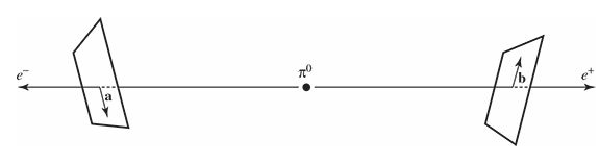
\includegraphics[width=0.75\textwidth]{figures/bell_scheme.eps}
    \caption{Belova postavka misaonog eksperimenta sa osama mjerenja koje mogu biti
        u proizvoljnim pravcima.}
    \label{fig:bell_exp_figure}
\end{figure}

Po\dj imo sada od pretpostavke da zaista postoji neka skrivena varijabla $\lambda$ koja omogućuje kompletniji opis stanja. Pošto se mjerenje može vršiti u bilo kojem pravcu, pretpostavimo da odabir pravca ne utiče na ishod mjerenja, već postoji neka funkcija koja je zavisna od skrivene varijable koja određuje ishod mjerenja.
Nazovimo funkciju koja određuje ishod mjerenja spina elektrona u pravcu $\vec{a}$, $A(\vec{a}, \lambda)$ i pozitorna u pravcu $\vec{b}$, $B(\vec{b}, \lambda)$.
Pošto ove funkcije utiču na ishod mjerenja, zaključujemo da su moguće njihove vrijednosti $\pm 1$.

Srednja vrijednost proizvoda pojedinačnih mjerenja je data sa

\begin{equation}
    P(\vec{a}, \vec{b}) = \int \rho (\lambda) A(\vec{a}, \lambda) B(\vec{b}, \lambda) d\lambda
\end{equation}
gdje smo sa $\rho (\lambda)$ označili gustinu vjerovatnoće skrivene varijable.
Ako posmatramo slučaj u kojem su detektori postavljeni u pravcima koji su međusobno paralelni, izmjerićemo uvijek suprotne spinove pa važi

\begin{equation}
    A(\vec{m}, \lambda) = - B(\vec{m}, \lambda).
\end{equation}
Srednja vrijednost proizvoda sada može da se napiše kao

\begin{equation}
    P(\vec{a}, \vec{b}) = - \int \rho (\lambda) A(\vec{a}, \lambda) A(\vec{b}, \lambda) d\lambda.
\end{equation}
Za bilo koji drugi jedinični vektor $\vec{c}$ važi takođe

\begin{equation}
    P(\vec{a}, \vec{c}) = - \int \rho (\lambda) A(\vec{a}, \lambda) A(\vec{c}, \lambda) d\lambda.
\end{equation}
Ako oduzmemo ove dvije jednačine dobijamo

\begin{equation}
    P(\vec{a}, \vec{b}) - P(\vec{a}, \vec{c})  = - \int \rho (\lambda) [A(\vec{a}, \lambda) A(\vec{b}, \lambda) - A(\vec{a}, \lambda) A(\vec{c}, \lambda) ] d\lambda.
\end{equation}
Zbog toga što je

\begin{equation}
    [A(\vec{b}, \lambda)]^2 = 1
\end{equation}
za proizvoljan vektor $\vec{b}$, drugi član u integrandu možemo pomnožiti sa takvom "jedinicom", pa dobijemo

\begin{equation}
    P(\vec{a}, \vec{b}) - P(\vec{a}, \vec{c})  = - \int \rho (\lambda) \left\{A(\vec{a}, \lambda) A(\vec{b}, \lambda) - A(\vec{a}, \lambda) A(\vec{c}, \lambda)[A(\vec{b}, \lambda)]^2 \right\}d\lambda.
\end{equation}
Jednostavnim izvlačenjem ispred zagrade dobijemo

\begin{equation}
    P(\vec{a}, \vec{b}) - P(\vec{a}, \vec{c})  = - \int \rho (\lambda) A(\vec{a}, \lambda) A(\vec{b}, \lambda) [1- A(\vec{c}, \lambda) A(\vec{b}, \lambda) ] d\lambda.
\end{equation}
Uzmimo sada apsolutnu vrijednost ovog izraza:

\begin{equation}
    \left|{P(\vec{a}, \vec{b}) - P(\vec{a}, \vec{c})}\right| =  \int \left| \rho (\lambda) A(\vec{a}, \lambda) A(\vec{b}, \lambda) [1- A(\vec{c}, \lambda) A(\vec{b}, \lambda)  ] \right| d\lambda.
\end{equation}
Pošto funkcije $A$ i $B$ uzimaju vrijednosti $\pm 1$ lako je vidjeti da je

\begin{equation}
    \left|A(\vec{a}, \lambda) A(\vec{b}, \lambda)\right| = 1.
\end{equation}

Analizirajmo sada član koji je preostao:

\begin{equation}
    \rho (\lambda)[1 - A(\vec{c}, \lambda) A(\vec{b}, \lambda) ].
\end{equation}
S obzirom da je $\rho(\lambda)$ gustina vjerovatnoće, kao takva funkcija mora biti ne-negativna tako da za taj član važi

\begin{equation}
    \rho(\lambda) \ge0 , \quad \forall \lambda.
\end{equation}
Proizvod $A(\vec{c}, \lambda) A(\vec{b}, \lambda)$ može imati vrijednosti $\pm 1$ tako da je

\begin{equation}
    1 - A(\vec{c}, \lambda) A(\vec{b}, \lambda) \ge 0 , \quad \forall \lambda.
\end{equation}
Dakle,

\begin{equation}
    \rho (\lambda)[1 - A(\vec{c}, \lambda) A(\vec{b}, \lambda) ] \ge 0, \quad \forall \lambda.
\end{equation}
Slijedi:


\begin{equation}
    \left|{P(\vec{a}, \vec{b}) - P(\vec{a}, \vec{c})}\right| \le  \int  \rho (\lambda)  [1- A(\vec{c}, \lambda) A(\vec{b}, \lambda)  ]  d\lambda = \underbrace{\int \rho(\lambda)d\lambda}_{1} + P(\vec{c}, \vec{b}).
\end{equation}
Konačno dobijemo Belovu nejednakost

\begin{equation}
    \left|{P(\vec{a}, \vec{b}) - P(\vec{a}, \vec{c})}\right| \le 1 +  P(\vec{c}, \vec{b}).
\end{equation}
Rezultat važi za bilo koju teoriju skrivenih varijabli, jer je $\rho(\lambda)$ proizvoljna funkcija raspodjele.

\section{Narušenje Belovih nejednakosti i implikacije}

Konstruišimo sada jednostavan primjer kojim možemo pokazati da dolazi do narušavanja Belovih nejednakosti. Na slici
su prikazana tri pravca u kojima možemo izvršiti mjerenje.

Želimo izračunati proizvod izmjerenih spinova po jednačini \eqref{eq:srednja_vrijednost_proizvoda}. Ako sa $\theta$ ozna\v cimo ugao me\dj u pravcima $\vec{a}$ i $\vec{b}$, onda se ova jedna\v cina mo\v ze napisati u obliku
\begin{equation}
    P(\vec{a},\vec{b}) = -cos\theta.
\end{equation}\\


% \begin{minipage}{0.6\textwidth}
% Your TikZ picture code here
\begin{tikzpicture}[scale=3, shift={(10,10)}]
    \def\arrowlength{1.5}

    % Arrow at 90 degrees
    \draw[->] (0,0) -- (\arrowlength,0) node[midway, below] {$\overrightarrow{b}$};

    % Arrow at 90 degrees
    \draw[->] (0,0) -- (0,\arrowlength) node[midway, left] {$\overrightarrow{a}$};

    \def\arrowlength{2}

    % Arrow at 45 degrees
    \draw[->] (0,0) -- (45:\arrowlength) node[midway, above, right] {$\overrightarrow{c}$};

    % draw arc
    \draw (0,0) -- (0.5,0) arc (0:45:0.5) -- cycle;
    \node at (0.3,0.15) {45\textdegree};
\end{tikzpicture}
\captionof{figure}{Detektori postavljeni sa relativnim uglovima od $45^\degree$ i $90^\degree$.}
\label{fig:detectors_with_chosen_angles}
% \end{minipage}

Ako izaberemo da ugao između pravaca $\vec{a}$ i $\vec{b}$ bude $90^\degree$, a uglovi ime\dj u pravaca $\vec{a}$ i $\vec{c}$, odnosno $\vec{b}$ i $\vec{c}$, po $45^\degree$ (slika: \ref{fig:detectors_with_chosen_angles}), Belova nejednakost glasi:
\begin{equation*}
    | cos(90^\degree) - cos(45^\degree)|\le 1 + cos(45^\degree).
\end{equation*}
Vidimo da ova nejednakost nije istinita, te zaključujemo da su Belove nejednakosti narušene.


\chapter{Eksperimentalno testiranje Belovih\\nejednakosti}


Eksperimenti za testiranje Belovih nejednakosti su izvedeni ve\' c 1960-ih i 1970-ih godina, a 2022. godine Nobelovu
nagradu su dobili Alen Aspekt (\textit{Alain Aspect}), D\v zon Klauzer (\textit{John Clauser}) i Anton Cajlinger (\textit{Anton Zeilinger}).

Oni su osmislili tri verzije eksperimenta u kojem se koriste polarizovani fotoni, umjesto raspada piona,
kako bi se testirale Belove nejednakosti. Da bi se isklju\v cilo "favorizovanje" određenih pravaca u eksperimentu, obje orijentacije su
postavljene kvazi-slu\v cajno nakon \v sto su fotoni ve\' c bili u letu.
Pokazalo se da su Belove nejednakosti u ovim eksperimentima naru\v sene, \v sto je zna\v cilo eksperimentalnu potvrdu
ispravnosti kvantne mehanike i propast "realizma" zbog nelokalnosti koju su eksperimenti potvrdili.

Hronolo\v ski, Klauzer je osmislio prvu verziju eksperimenta \v cija je 
su\v stina u slanju dva polarizovana spregnuta fotona, dobijena koriste\' ci atome Ca, u opozitnim smjerovima prema filterima kroz koje
\' ce foton ili pro\' ci ili ne\' ce, \v sto zavisi od ugla pod kojim je filter postavljen
i kako je foton polarizovan.

U momentu kreiranja para fotona ne mo\v zemo znati kakva im je polarizacija, ve\' c samo to da su im
polarizacije paralelne. To zna\v ci da ako su filteri postavljeni paralelno, u slu\v caju da jedan foton pro\dj e, vjerovatno\' ca da \' ce pro\' ci i drugi je $1$.
Ako je ugao izme\dj u filtera $\dfrac{\pi}{2}$ uvijek \' ce jedan foton pro\' ci, a drugi ne.

Zanimljivi efekti se vide ako se posmatraju uglovi filtera ba\v s izme\dj u $0$ i $\dfrac{\pi}{2}$. Tada rezultati variraju,
pa ponekad pro\dj u oba fotona, ponekad samo jedan, a u nekim slu\v cajevima nijedan.

Kada se uradi dosta mjerenja i zabilje\v ze se rezultati, mo\v ze se uo\v citi korelacija koja je mnogo ve\'ca nego kada bi
proces bio vo\dj en pod uticajem neke skrivene varijable pri \v cemu bi polarizacije fotona ve\'c bile predeterminisane u momentu njihove kreacije, a ne u trenutku mjerenja.

Ovaj eksperiment je unaprije\dj ena verzija misaonog Belovog eksperimenta, jer se koriste i detektori koji
detektuju fotone koji nisu uspjeli pro\'ci kroz filter, pa je samim tim eksperiment potpuniji i rezultat precizniji (slika \ref{fig:chsh_scheme}).
U svojoj sr\v zi ovaj eksperiment nosi korelacionu funkciju koja ima zadatak da modeluje odgovor na pitanje: "Koliko
\v cesto \'ce oba fotona pro\' ci kroz filtere, a koliko \v cesto samo jedan?", koja je ograni\v cena odozgo i predstavlja analognu formu
Belovih nejednakosti, zvanu CHSH nejednakost.

\begin{figure}
    \centering
    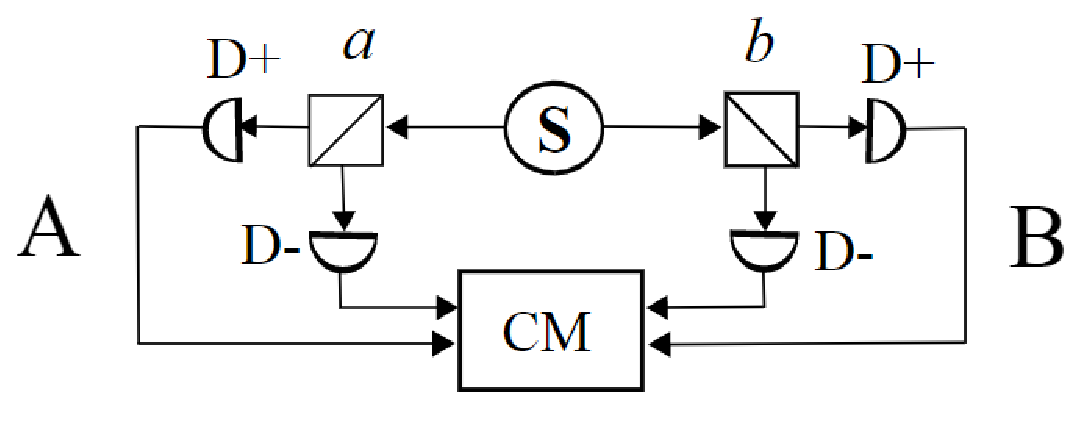
\includegraphics[width=0.75\textwidth]{figures/chsh_scheme.eps}
    \caption{Izvor \textit{S} emituje spregnute fotone koji potom odlaze u suprotnim smjerovima. U zavisnosti od njihove polarizacije i orijentacije filtera sti\'ci \' ce do  detektora $D_+$ ili $D_-$.
    Korelacija izme\dj u pojedina\v cnih mjerenja se mo\v ze izra\v cunati tako \v sto
    na\dj emo broj koji predstavlja odnos sume mjerenja pri kojima smo dobili rezultat da su oba fotona pro\v sla ili oba nisu pro\v sla kroz filter
    od koje smo oduzeli sumu mjerenja pri kojima je samo jedan od fotona pro\v sao kroz filter i ukupnog broja mjerenja, tj.
       $E(a,b) = N_{++} + N_{--} - (N_{+-} + N_{-+})/N$}
    \label{fig:chsh_scheme}
\end{figure}

Osim naru\v senja Belovih nejednakosti, novi potencijal za skladi\v stenje, preno\v senje i procesuiranje informacija je uvi\dj en sa novom verzijom eksperimenta, koju je osmislio Aspekt.
Konfiguracija eksperimenta je bila druga\v cija  u odnosu na Klauzerov u novom na\v cinu pobu\dj ivanja atoma tako da je frekvencija emitovanja
spregnutih fotona bila ve\'ca. Tako\dj e je kori\v sten kristal kvarca koji je slu\v zio za preusmjerenje fotona ka razli\v cito orijentisanim filterima.

Zanimljiv efekat se mogao vidjeti u slu\v caju kada se spregnuti par \v cestica (\v cestice $1$ i $2$) kre\' ce u suprotnim smjerovima i jedna od tih \v cestica nai\dj e na tre\'cu, slobodnu \v cesticu (\v cestica $3$).
U tom slu\v caju \v cestice $2$ i $3$ postaju spregnute, pri tome \v cestica $3$ gubi sve informacije o prethodnom stanju, ali se istovremeno to stanje "prepisuje" na \v cesticu $1$ koja
nikada nije ni do\v sla u kontakt sa \v cesticom $3$. Ovaj proces je poznat pod imenom \textit{kvatna teleportacija}.

Kvantna teleportacija je za sada jedini mehanizam kojim se nepoznato kvantno stanje (\textit{kvantna informacija}) mo\v ze u potpunosti prenijeti iz jednog u drugi sistem,
bez ikakvih gubitaka informacija. Nemogu\'ce je izmjeriti sve karakteristike sistema i poslati te informacije na drugu lokaciju, kako bi se
prvobitni sistem rekonstruisao, primarno zbog kolapsa talasne funkcije pri vr\v senju bilo kakvog mjerenja.

Nakon \v sto je kvantna teleportacija eksperimentalno pokazana, Cajlingerov eksperiment je dodao novu "dimenziju" eksperimentu i pokazao
mogu\' cnost sprezanja \v cestica koje su udaljene i nikada nisu do\v sle u kontakt.
Dva para (par \textit{A} i par \textit{B}) spregnutih \v cestica se emituju iz izvora. Nakon nekog vremena po jedna od \v cestica iz svakog para konvergiraju ka
ure\dj aju koji \' ce nekom transformacijom da u\v cini te dvije \v cestice spregnutima. Zbog kvantne teleportacije kvantne informacije preostalih
\v cestica \' ce se "prepisati" jedna na drugu i one \'ce postati spregnute iako nikada nisu do\v sle u kontakt.


\chapter{Zaključak}

Svi dosadašnji eksperimeni kojima su testirane Belove nejednakosti su pokazali da su one narušene, što predstavlja eksperimentalnu potvrdu ispravnosti kvantne mehanike i propast "realizma" zbog njegove pretpostavke o lokalnosti.

S druge strane ideja o nelokalnosti (u kontekstu superluminalnog uticaja) je svakako uznemiruju\' ca jer je toliko druga\v cija od onoga \v sto nam intuicija govori i ima neprihvatljive implikacije.
Prema specijalnoj teoriji relativnosti, postoje inercijalni sistemi u kojima se takav signal \v siri unazad u vremenu, pa bi efekti prethodili sopstvenim uzrocima - \v sto dovodi do
razli\v citih logi\v ckih anomalija.
Pitanje je da li su efekti posmatrani u ovim eksperimentima kauzalni, ili su dovoljno eteri\v cni da se izbjegne filozofski odgovor i da superluminalni uticaji u tom slu\v caju
dobiju novi interpretaciju.

Jedan od takvih primjera eteri\v cnih efekata bila bi sjenka bube koja preleti preko svjetlosnog snopa filmskog projektora (slika \ref{fig:bug_on_screen}). Udaljenost do ekrana mo\v ze biti proizvoljna, pa samim tim i brzina sjenke
mo\v ze biti proizvoljno velika, tako da mo\v zemo zamisliti scenario u kojem se sjenka bube kre\' ce brzinom ve\' com od brzine svjetlosti.
Ono \v sto ovdje moramo primjetiti je da sjenka ne nosi nikakvu energiju, niti prenosi bilo kakvu informaciju s jedne ta\v cke na drugu, tako da mi ne mo\v zemo iz ta\v cke $X$ prouzrokovati bilo
\v sta u ta\v cki $Y$ manipulacijom prolazne sjenke.

\begin{figure}[H]
    \centering
    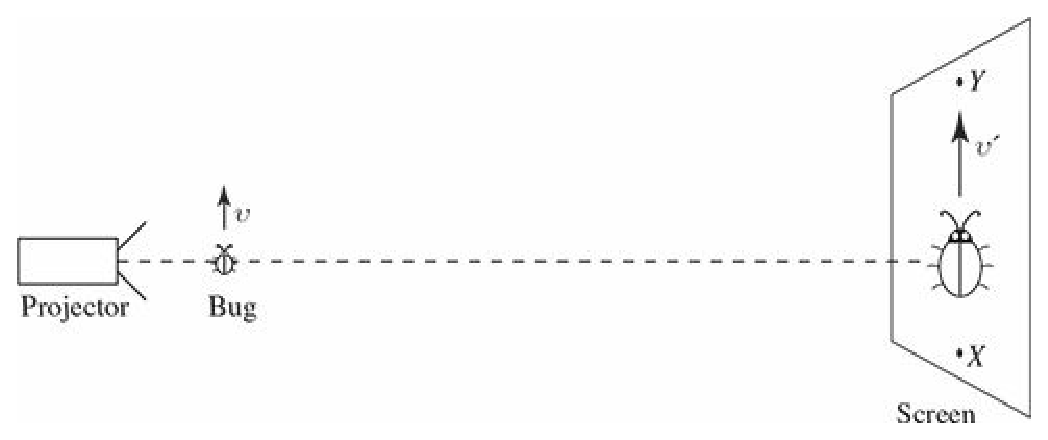
\includegraphics[width=0.75\textwidth]{figures/bug_on_screen.eps}
    \caption{Buba se kre\' ce brzinom $v$ preko svjetlosnog snopa filmskog projektora. U zavisnosti od udaljenosti platna, brzina $v'$ mo\v ze biti proivoljno velika.}
    \label{fig:bug_on_screen}
\end{figure}

O\v cigledno je da u Belovom eksperimentu postoji korelacija u podacima, s tim \v sto tu korelaciju mo\v zemo da vidimo
samo nakon \v sto uporedimo dva seta podataka (nakon \v sto su oba mjerenja zavr\v sena).
U skladu sa tim, odgovor na pitanje: "Da li mjerenje elektrona uti\v ce na sa njim spregnuti pozitron", je {\it{da}}, ali ne u obi\v cnom smislu te rije\v ci.
Da je odgovor negativan, ne bismo mogli objasniti korelacije u podacima.

Osoba koja vr\v si eksperiment, mo\v ze jedino da kontroli\v se da li \' ce izvr\v siti mjerenje ili ne, ali ne mo\v ze uticati na njegov ishod i ti rezultati su prakti\v cno
nasumi\v cni (ako se posmatraju odvojeno od rezulatata eksperimenata sa spregnutom \v cesticom) i ona ne mo\v ze koristiti svoje mjerenje da po\v salje signal osobi
na detektoru spregnute \v cestice (ne mo\v ze natjerati datu \v cesticu da promijeni spin, kao \v sto ni osoba u $X$ ne mo\v ze da uti\v ce na sjenku bube).

Ovo nas navodi da razlikujemo dvije vrste uticaja: "uzro\v cne" vrste i "eteri\v cne" vrste.
Uzro\v cne mo\v zemo detektovati vr\v se\' ci mjerenje na samom podsistemu, dok je za eteri\v cne, koje ne prenose informacije ili energiju, jedini dokaz
korelacija u podacima dobijenim eksperimentima na dva razli\v cita podsistema.
Uzro\v cni uticaji se ne mogu \v siriti superluminalnim brzinama, tj. princip lokalnosti za njih i dalje važi, ali zasad ne postoji razlog za\v sto bi to moralo da va\v zi za eteri\v cne.
\chapter{Dodatak}
\section{Srednja vrijednost proizvoda komponenti spinova dvaju \v cestica u proizvoljnim pravcima}

Posmatrajmo dvije čestice spina-$1/2$ u singletnom stanju opisanom vektorom:

\begin{equation}
    | 00 \rangle = \frac{1}{\sqrt2}(| \updownarrows \; \rangle - | \downuparrows \; \rangle) \label{eq:singletno_stanje}.
\end{equation}
Neka je $S_k^{(n)}$ operator komponente spina čestice $n \ (n = 1, 2)$ u pravcu k. Da bismo izračunali srednju vrijednost proizvoda komponentni spinova dvaju čestica u proizvoljnim pravcima zadatim ortovima $\vec{a}$ (za prvu česticu) i $\vec{b}$ (za drugu česticu), odredićemo prvo djelovanje proizvoda operatora tih komponenti na stanje (\ref{eq:singletno_stanje}).
Pošto govorimo o proizvoljnim pravcima izaberimo ih tako da se pravac $\vec{a}$ poklapa sa $z$ osom, a pravac $\vec{b}$ neka leži u $xz$ ravni:
\begin{equation*}
    S_a^{(1)} = S_z^{(1)} \quad S_b^{(2)} = cos{\theta} S_z^{(2)} + sin{\theta} S_x^{(2)}.
\end{equation*}

Da bismo odredili djelovanje proizvoda operatora $\hat{S}_a^{(1)}$
i $\hat{S}_b^{(2)}$ na stanje \eqref{eq:singletno_stanje}, potrebno je da znamo kako
operatori $\hat{S}_x^{(n)}$ i $\hat{S}_z^{(n)}$ djeluju na spinska
stanja $|\!\uparrow\;\!\rangle$ i $|\!\downarrow\;\!\rangle$
$n$-te \v cestice. Po\v sto su ova stanja svojstvena stanja
operatora $\hat{S}_z^{(n)}$, imamo
\begin{equation}
\hat{S}_z^{(n)} |\!\uparrow\;\!\rangle = \frac{\hbar}{2}\,
|\!\uparrow\;\!\rangle, \quad \hat{S}_z^{(n)}
|\!\downarrow\;\!\rangle = -\frac{\hbar}{2}\,
|\!\downarrow\;\!\rangle. \label{Sz.spin.st}
\end{equation}
S druge strane, djelovanje operatora $\hat{S}_x^{(n)}$ na spinska
stanja dobijamo polaze\'ci od djelovanja operatora podizanja i
spu\v stanja $\hat{S}_\pm^{(n)} = \hat{S}_x^{(n)} \pm i
\hat{S}_y^{(n)}$ na njih, koje glasi
\begin{equation}
\hat{S}_+^{(n)} |\!\uparrow\;\!\rangle = 0, \quad \hat{S}_-^{(n)}
|\!\uparrow\;\!\rangle = \hbar\, |\!\downarrow\;\!\rangle,
\end{equation}
\begin{equation}
\hat{S}_+^{(n)} |\!\downarrow\;\!\rangle = \hbar\,
|\!\uparrow\;\!\rangle, \quad \hat{S}_-^{(n)}
|\!\downarrow\;\!\rangle = 0,
\end{equation}
odnosno
\begin{equation}
(\hat{S}_x^{(n)} + i \hat{S}_y^{(n)}) |\!\uparrow\;\!\rangle = 0,
\quad (\hat{S}_x^{(n)} - i \hat{S}_y^{(n)}) |\!\uparrow\;\!\rangle
= \hbar\, |\!\downarrow\;\!\rangle,
\end{equation}
\begin{equation}
(\hat{S}_x^{(n)} + i \hat{S}_y^{(n)}) |\!\downarrow\;\!\rangle =
\hbar\, |\!\uparrow\;\!\rangle, \quad (\hat{S}_x^{(n)} - i
\hat{S}_y^{(n)}) |\!\downarrow\;\!\rangle = 0.
\end{equation}
Sabiranjem odvojeno prve dvije i druge dvije jedna\v cine
neposredno slijedi
\begin{equation}
\hat{S}_x^{(n)} |\!\uparrow\;\!\rangle = \frac{\hbar}{2}\,
|\!\downarrow\;\!\rangle, \quad \hat{S}_x^{(n)}
|\!\downarrow\;\!\rangle = \frac{\hbar}{2}\,
|\!\uparrow\;\!\rangle. \label{Sx.spin.st}
\end{equation}

Koriste\'ci rezultate (\ref{Sz.spin.st}) i (\ref{Sx.spin.st})
dalje imamo:

\begin{equation}
    \begin{aligned}
        S_a^{(1)}S_b^{(2)} | 00 \rangle & = S_z^{(1)}\left(cos{\theta} S_z^{(2)} + sin{\theta} S_x^{(2)}\right) \left[\frac{1}{\sqrt2}(| \updownarrows \; \rangle - | \downuparrows \; \rangle)\right]                                                                                                                                                                  \\[1ex]
                                        & = \frac{1}{\sqrt{2}} \left[ S_z^{(1)}|\uparrow\rangle \left( cos{\theta} S_z^{(2)}|\downarrow\rangle + sin{\theta} S_x^{(2)}|\downarrow\rangle \right) - S_z^{(1)}|\downarrow\rangle \left( cos{\theta} S_z^{(2)}|\uparrow\rangle + sin{\theta} S_x^{(2)}|\uparrow\rangle \right) \right]                                     \\[1ex]
                                        & = \frac{1}{\sqrt{2}} \left[ \frac{\hbar}{2}|\uparrow\rangle \left( -cos{\theta}\frac{\hbar}{2}|\downarrow\rangle + sin{\theta} \frac{\hbar}{2}|\uparrow\rangle \right) + \frac{\hbar}{2}|\downarrow\rangle \left( cos{\theta} \frac{\hbar}{2}|\uparrow\rangle + sin{\theta} \frac{\hbar}{2}|\downarrow\rangle \right) \right] \\[1ex]
                                        & = \frac{\hbar^2}{4\sqrt{2}} \left[ -cos{\theta} |\updownarrows\rangle + sin{\theta}|\upuparrows\rangle + cos{\theta} |\downuparrows\rangle + sin{\theta}|\downdownarrows\rangle \right]                                                                                                                                       \\[1ex]
                                        & = \frac{\hbar^2}{4} \left[ - cos{\theta} \frac{1}{\sqrt{2}} \left( |\updownarrows\rangle -  |\downuparrows\rangle \right) + sin{\theta} \frac{1}{\sqrt{2}} \left( |\upuparrows\rangle + |\downdownarrows\rangle \right) \right]                                                                                               \\[1ex]
                                        & = \frac{\hbar^2}{4} \left[ - cos{\theta}|00\rangle + sin{\theta} \frac{1}{\sqrt{2}} \left( | 11 \rangle + | 1 {-1} \rangle \right) \right].
    \end{aligned}
\end{equation}
Prema tome očekivana vrijednost proizvoda spin komponenti je:

\begin{equation}
    \langle  S_a^{(1)}S_b^{(2)} \rangle = \frac{\hbar^2}{4} \langle 00 | \left[ - cos{\theta}|00\rangle + sin{\theta} \frac{1}{\sqrt{2}} \left( | 11 \rangle + | 1 {-1} \rangle \right) \right]
\end{equation}
što se zbog ortonormiranosti stanja $| 00 \rangle,| 11 \rangle,| 10 \rangle,| 1{-1}\rangle$ svodi na:

\begin{equation}
    \langle  S_a^{(1)}S_b^{(2)} \rangle = -\frac{\hbar^2}{4}cos{\theta},
\end{equation}
odnosno

\begin{equation}
    \langle  S_a^{(1)}S_b^{(2)} \rangle = -\frac{\hbar^2}{4} \vec{a} \cdot \vec{b}.
\end{equation}

U svrhu našeg misaonog eksperimenta mjerenje ćemo vršiti u jedinicama $\dfrac{\hbar}{2}$, pa ćemo uzeti da je srednja vrijednost proizvoda komponenti spinova u proizvoljnim pravcima:

\begin{equation}
    P(\vec{a}, \vec{b}) = - \vec{a} \cdot \vec{b}.
\end{equation}
\chapter*{Literatura}

\addcontentsline{toc}{chapter}{Literatura}

\begin{enumerate}

\item A. Einstein, B. Podolsky and N. Rosen, \textit{Can
Quantum-Mechanical Description of Physical Reality Be Considered
Complete?}, Phys. Rev. \textbf{47}, 777 (1935)

\item N. Bohr, \textit{Can Quantum-Mechanical Description of
Physical Reality Be Considered Complete?}, Phys. Rev. \textbf{48},
696 (1935)

\item D. Bohm and Y. Aharonov, \textit{Discussion of Experimental
Proof for the Paradox of Einstein, Rosen, and Podolsky}, Phys.
Rev. \textbf{108}, 1070 (1957)

\item J. S. Bell, \textit{On the Einstein Podolsky Rosen paradox},
Physics \textbf{1}, 195 (1964)

\item D. J. Griffiths, \textit{Introduction to Quantum Mechanics}
(Prentice Hall, Upper Sadle River, New Jersey, 1995)

\item B. H. Bransden and C. J. Joachain, \textit{Quantum
Mechanics}, 2nd edition (Pearson, Prentice Hall, Harrlow, England,
2000)

\item The Nobel Prize in Physics 2022, Popular science background:
How entanglement has become a powerful tool (The Royal Swedish
Academy of Sciences, 4 October 2022),
\textsf{https:/\!/www.nobelprize.org/uploads/2022/10/popular-physicsprize2022-3.pdf}

\item Scientific Background on the Nobel Prize in Physics 2022
"for experiments with entangled photons, establishing the
violation of Bell inequalities and pioneering quantum information
science" (The Royal Swedish Academy of Sciences, 4 October 2022),
\textsf{https:/\!/www.nobelprize.org/uploads/2023/10/advanced-physicsprize2022-4.pdf}

\end{enumerate}

\end{document}
